\chapter{Chọn thân máy và các chi tiết phụ}
\section{Chọn thân máy}
\subsection{Yêu cầu}
\begin{itemize}
    \item Chỉ tiêu cơ bản của hộp giảm tốc là khối lượng nhỏ và độ cứng cao.
    \item Vật liệu làm vỏ là gang xám GX15-32.
    \item Hộp giảm tốc bao gồm: thành hộp, nẹp hoặc gân, mặt bích, gối đỡ, \ldots
    \item Bề mặt lắp ghép giữa nắp và thân được cạo sạch hoặc mài để lắp sít, khi lắp có một lớp sơn mỏng hoặc sơn đặc biệt.
    \item Chọn bề mặt ghép nắp và thân: song song mặt đế.
    \item Mặt đáy về phía lỗ tháo dầu với độ dốc khoảng $2^\circ$ và ngay tại chỗ tháo dầu lõm xuống.
\end{itemize}

\subsection{Xác định kích thước vỏ hộp}

\begin{table}[H]
    \centering
    \begin{tabular}{|p{5cm}|c|p{7cm}|} % Cột đầu tiên cố định độ rộng 5cm
    \hline
    \textbf{Tên gọi} & \textbf{Ký hiệu} & \textbf{Giá trị số bộ} \\
    \hline
    Chiều dày thân hộp & $\delta$ & $0.02a + 1 = 5$, nhỏ hơn 7mm $\rightarrow$ chọn $\delta = 10$mm \\
    \hline
    Chiều dày nắp hộp & $\delta_i$ & $\delta_i \approx \delta = 10$mm \\
    \hline
    Chiều dày mặt bích thân hộp & $s_2$ & $2.35\delta = 23.5$mm \\
    \hline
    Chiều dày mặt bích nắp hộp & $s_1$ & $1.5\delta_i = 15$mm \\
    \hline
    Đường kính bu lông nền & $d_1$ & $0.03a + 12 = 16.8$mm \\
    \hline
    Số bu lông nền & $z$ & 4 \\
    \hline
    Đường kính bu lông tại vị trí lắp ổ lăn & $d_2$ & $0.75d_1 = 12.6$mm, theo tiêu chuẩn chọn bu lông M14 \\
    \hline
    Đường kính bu lông tại vị trí lắp thân hộp với nắp hộp & $d_3$ & $0.6d_1 = 10.08$mm, theo tiêu chuẩn chọn bu lông M12 \\
    \hline
    Chiều rộng mặt bích & $S$ & $k + 1.5\delta = 40 + 15 = 55$, $k$ chọn theo bu lông nền (M16 ứng với $k=40$, chọn theo bảng 10.1 [1]) \\
    \hline
    Chiều dày gân tăng cứng thân hộp & $\delta_3$ & $(0.8 \ldots 1)\delta \rightarrow$ chọn $\delta_3 = 10$mm \\
    \hline
    Khe hở nhỏ nhất giữa bánh răng và thân hộp & $c_2$ & $c_2 = 1.2\delta = 12$mm \\
    \hline
    Vị trí tuyến bu lông tại nơi độ và mặt bích thân hộp & $c$ & $c \approx (1 \ldots 1.2)d_2 = 14$mm \\
    \hline
    Khoảng cách từ mặt đáy thân hộp đến định bằng răng & $Y$ & $Y = 4.8\delta = 48$mm \\
    \hline
    Chiều dày nắp và thân HGT tại vị trí lắp ổ & & Chọn theo kết cấu sao cho lớn hơn hoặc bằng $(s_1 + s_2)$ \\
    \hline
    \end{tabular}
    \end{table}
\subsection{Kích thước nắp ổ}
Chọn theo đường kính ngoài của ổ lăn, thông số của các nắp ổ được thể hiện \\qua bảng sau:
\begin{table}[H]
    \centering
    \begin{tabular}{|l|c|c|c|c|c|c|}
    \hline
    \textbf{Trục} & \textbf{$D1$} & \textbf{$D2$} & \textbf{$D3$} & \textbf{$n$} & \textbf{$d$} & \textbf{$d1$} \\
    \hline
    I & 90 & 110 & 62 & 4 & 9 & 15 \\
    \hline
    II & 110 & 130 & 80 & 6 & 9 & 15 \\
    \hline
    \end{tabular}
\end{table}
\cleardoublepage
\section{Các chi tiết hệ thống bôi trơn hộp giảm tốc}
\subsection{Que thăm dầu}
Chọn que thăm dầu M16x1.5 với thông số sau:
\begin{table}[H]
    \centering
    \begin{tabular}{|c|c|c|c|c|c|c|c|c|}
    \hline
    $\mathbf{d}$ & $\mathbf{d1}$ & $\mathbf{d2}$ & $\mathbf{D}$ & $\mathbf{D1}$ & $\mathbf{L1}$ & $\mathbf{l}$ & $\mathbf{l1}$ & $\mathbf{b}$ \\
    \hline
    M16x1.5 & 5 & 7 & 24 & 16 & 40 & 16 & 8 & 4 \\
    \hline
    \end{tabular}
\end{table}
\begin{figure}[H]
    \centering
    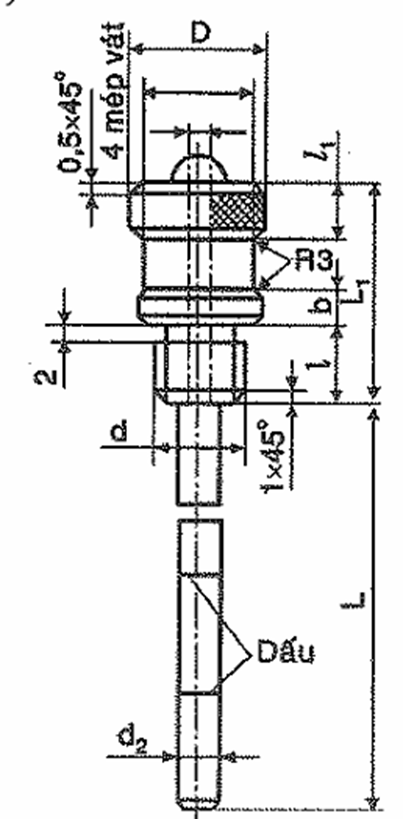
\includegraphics[width=0.5\textwidth]{pictures/quethamdau.png}
\end{figure}
\cleardoublepage
\subsection{Nút tháo dầu}
Chọn nút tháo dầu dạng vít ren trụ tròn M20x1.5 với thông số như sau:
\begin{table}[H]
    \centering
    \begin{tabular}{|c|c|c|c|c|c|c|c|c|c|c|}
    \hline
    $\mathbf{d1}$ & $\mathbf{D}$ & $\mathbf{D1}$ & $\mathbf{L}$ & $\mathbf{l}$ & $\mathbf{b}$ & $\mathbf{s}$ & $\mathbf{t}$ & $\mathbf{d2}$ & $\mathbf{D2}$ & $\mathbf{D2}$ \\
    \hline
    M20x1.5 & 30 & 25.4 & 30 & 15 & 4 & 22 & 2.5 & 20 & 32 & 3 \\
    \hline
    \end{tabular}
\end{table}
\begin{figure}[H]
    \centering
    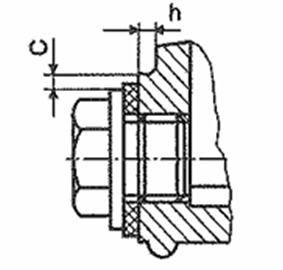
\includegraphics[width=0.5\textwidth]{pictures/nut.png}
\end{figure}

\subsection{Cửa thăm và nút thông hơi}
Chọn nắp cửa thăm và nút thông hơi có kích thước như sau:
\begin{center}
\begin{tabular}{|c|c|c|c|c|c|c|c|c|}
\hline
A & B & A1 & B1 & C & K & R & Dimension & Quantity \\
\hline
40 & 40 & 80 & 90 & 65 & 30 & 10 & M8 & 4 \\
\hline
\end{tabular}
\end{center}
\begin{figure}[H]
    \centering
    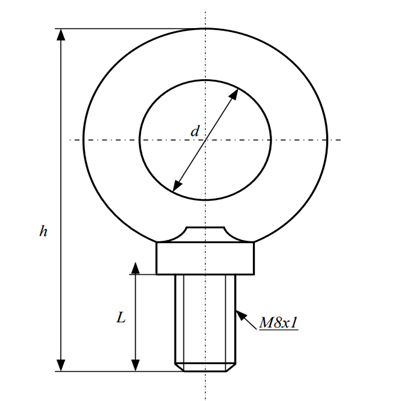
\includegraphics[width=0.5\textwidth]{pictures/vitvong.png}
\end{figure}
\subsection{Vòng chắn dầu}
Gồm 3 rãnh tiết diện tam giác đều có góc ở đỉnh là 60 độ, khoảng cách giữa các đỉnh là 3mm. Mép ngoài của vòng cách thành trong của hộp một khoảng bằng 3mm. 
\begin{figure}[H]
    \centering
    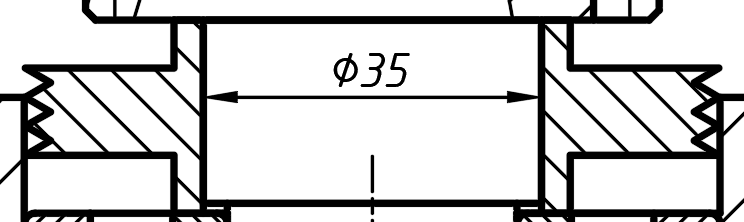
\includegraphics[width=0.5\textwidth]{pictures/vongchandau.png}
\end{figure}
\subsection{Chốt định vị}
Dùng để xác định vị trí làm việc êm của hộp giảm tốc sau khi lắp ráp, hình dạng và kích thước được cho bởi:
\begin{figure}[H]
    \centering
    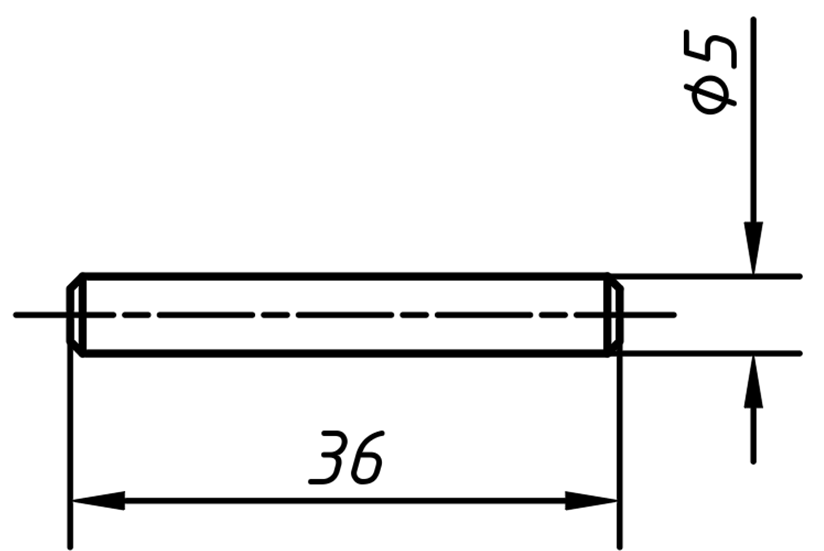
\includegraphics[width=0.5\textwidth]{pictures/chotdinhvi.png}
\end{figure}
\subsection{Vòng phớt}
Vòng phớt là loại lót kín động gián tiếp nhằm mục đích bảo vệ ổ khỏi bụi bặm, chất bẩn, hạt cứng và các tạp chất khác xâm nhập vào ổ. Những chất này làm ổ chóng bị mài mòn và bị han gỉ. Ngoài ra, vòng phớt còn đề phòng dầu chảy ra ngoài. Tuổi thọ ổ lăn phụ thuộc rất nhiều vào vòng phớt. Vòng phớt được dùng khá rộng rãi do có kết cấu đơn giản, thay thế dễ dàng. Tuy nhiên có nhược điểm là chóng mòn và ma sát lớn khi bề mặt trục có độ nhám cao.\\
Theo tiêu chuẩn, chọn vòng phớt có đường kính trong là 25mm cho trục dẫn và vòng phớt có đường kính trong là 38mm cho trục bị dẫn. Các kích thước khác của vòng phớt được lấy theo tiêu chuẩn.
\begin{figure}[H]
    \centering
    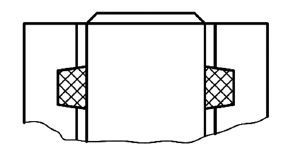
\includegraphics[width=0.5\textwidth]{pictures/vongphot.png}
\end{figure}
\cleardoublepage